
\section{Monte Carlo Simulation}
\label{sec:cmsexperiment:simulation}



The Monte Carlo simulated events are produced via a pipeline which can be divided into three main stages, the event generation (GEN), the detector simulation (SIM), and the digitization (DIGI). Then the same reconstruction and triggering algorithms used for data are applied to simulated events.


\begin{figure}[ht]
    \centering
    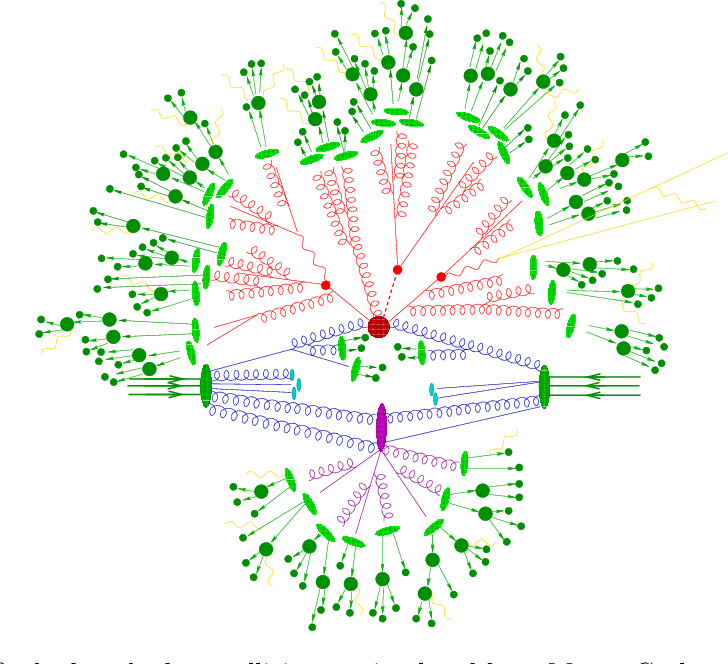
\includegraphics[trim={0 0.1cm 0 0}, clip, width=0.6\textwidth]{chapters/CMSExperiment/sectionMCSimulation/figures/ps.png}
    \caption{Physics processes happening in a proton-proton collision. The lower purple blob represents underline events. The upper purple blob shows the hard process with ISR before it and with FSR-PS-hadronization-decay after it. All of these processes are handled properly in the GEN stage by the generator and Pythia8. }
    \label{fig:cmsexperiment:simulation:collision}
\end{figure}


% GEN
The GEN stage generates a set of final-state particles for each event according to the interested QFT physics model. The involved software can be summarized as ``Generator+\PYTHIA". Common generators include \MADGRAPH, \POWHEG, \HERWIG, \SHERPA. The event generation starts with initiating the generator with a configuration of the key input information, such as the beam parameters, the parton distribution functions (PDFs), and the corresponding QFT models.  Upon initialized, the generator calculates the matrix element and cross-section of the hard processes at some perturbative order according to the provided QFT models. Then it outputs Monte Carlo events from the calculated differential cross-section. Possible QCD and QED ISR/FSR are also included in the generated events. Next, for all particles from the generator, \PYTHIA is used to perform the potential parton showering, hadronization, and decay of unstable particles. In addition, \PYTHIA also adds underline events (UE) to the generated events according to certain UE tuning. The underline events are QCD scatterings at the same proton-proton vertex as the hard process. Figure~\ref{fig:cmsexperiment:simulation:collision} illustrates the physics processes happening during a proton-proton collision, all of which are properly treated in the GEN stage with the ``Generator+\PYTHIA" setup.




% sim
The SIM stage uses GEANT4 to simulate the energy deposits, known as hits, of the final state particles in the CMS detector. To achieve this, a detailed geometry model of the CMS detector, including the information about the detector layout, the magnetic field, the electronics, the cables, and the supporting mechanics, is created in the GEANT4. With this geometry modelling, GEANT4 simulates the hits based on the physics for the interaction between the particles and the materials. After GEN-SIM, the pile-up events, often referred to as MinBias (MB) events and separately produced beforehand with the same GEN-SIM pipeline, are mixed with the signal events according to the instant luminosity and expected average number of PUs.

% digi reco
The DIGI stage simulates the response of the detector readout electronics to hits. The purpose is to simulate the best realism of the collected digitized signal as close as possible to the real CMS detector. After the DIGI stage, the same reconstruction and triggering software as the data events are used for the MC events. Finally, the MC events are output and stored in the same format as the experimental data as well.